    \section{Calcolare il campo elettrostatico di una distribuzione
    	piana ed uniforme di carica elettrica mediante il teorema di
    	Gauss.}
    Per distribuzione piana e uniforme di carica si intende una distribuzione di cariche su un piano nel piano $xyz$ dove vi \`e una densit\'a piana di carica $\sigma$ costante per tutto il filo.
    Si noti che :
    $$ \left[\sigma\right] =  \left[\frac{Q}{m^2}\right] $$
    
    Secondo il teorema di Gauss per il campo elettrico, vale quanto segue:
    \begin{displaymath}
    \Phi_S\left(\vec{E}\right) = \oint_{S}{\vec{E} \cdot \hat{n}} = \frac{\sum{Q_{interne}}}{\varepsilon_0}
    \end{displaymath}
    
    Per calcolare il flusso del campo elettrico su tale distribuzione occorre quindi scegliere una opportuna superfcie chiusa, per esempio un cilindro di altezza $h$ e raggio $r$ tale che intersechi il perpendicolarmente la distribuzione piana.
    
    \begin{center}
    	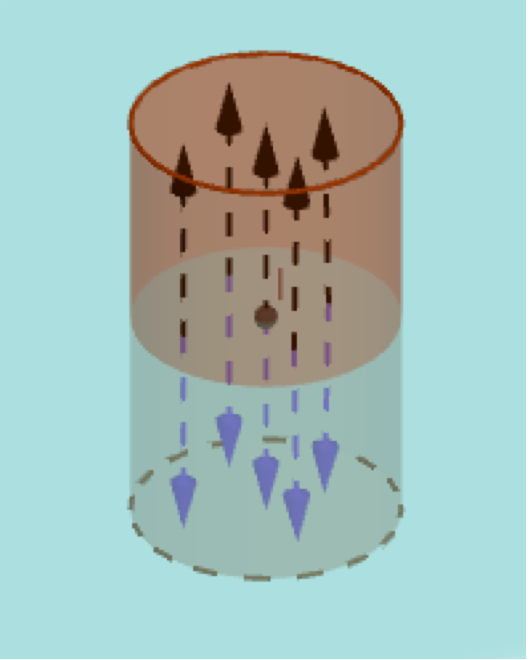
\includegraphics[height=150pt]{dpcarica}\\
    	\textbf{Esempio grafico :} scelta della superficie
    \end{center}
    
    \pagebreak
    In tale figura il contributo del campo elettrico al flusso \`e nullo per la superficie laterale del cilindro (dove le linee di campo sono parallele), mentre \`e massimo per la superficie delle basi (in quanto ogni suo punto \`e normale alla linea di campo elettrico). Pertanto si ha che:
    $$ S = 2 S_{base} = 2 \pi r^2 $$
    $$ \sum{Q_{interne}} = \sigma S_{base} $$
    $$ \Phi_S\left(\vec{E}\right) = \frac{\sum{Q_{interne}}}{\varepsilon_0} = \oint_{S}{\vec{E} \cdot \hat{n}} $$
    $$ \oint_{S}{\vec{E} \cdot \hat{n}} = 2|\vec{E}| S_{base} $$
    $$ \frac{\sigma \cancel{S_{base}}}{\varepsilon_0} = 2|\vec{E}| \cancel{S_{base}} $$
	$$ |\vec{E}| = \frac{\sigma}{2 \varepsilon_0} $$
	
	$\hfill\square$